\chapter{Conclusioni}
%\markboth{Introduzione}{Introduzione}
\label{cap:conclusioni}


\begin{figure}
\centering
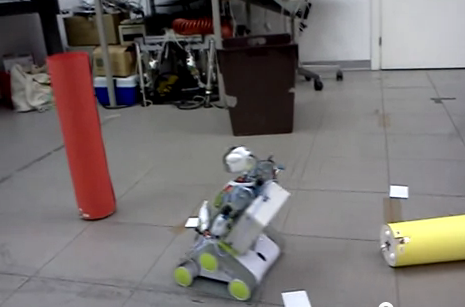
\includegraphics[scale=0.7]{images/attaccotorre}
\caption{Spykee va all'attacco della torre, dopo aver distrutto una fabbrica}
\end{figure}

Dalle prove effettuate, il gioco risulta sufficientemente giocabile e coinvolgente per il giocatore, anche in un'area di gioco di dimensione limitata.

Alcune problematiche relative all'implementazione del gioco sono dovute ai limiti dell'hardware a disposizione. In particolare, il funzionamento dell'algoritmo di visione è fortemente penalizzato dalla bassa qualità dell'immagine proveniente dalla telecamera (sia dalla bassa risoluzione che, soprattutto, dall'enorme compressione JPEG che viene effettuata da Spykee prima di inviare l'immagine via rete). Altri problemi della visione sono legati alla forte dipendenza alle condizioni di luminosità dell'algoritmo di visione utilizzato, che rende necessario effettuare più volte il training del classificatore, a seconda delle condizioni di luce.

%Le maggiori problematiche nell'implementazione del gioco sono dovute ai limiti dell'hardware: in particolare la visione e il controllo del movimento. 

%La visione è penalizzata sia dalla bassa risoluzione dell'immagine sia dalla forte compressione jpeg a cui è sottoposta (e che purtroppo non può essere evitata). Questo rende l'individuazione dei blob imprecisa e difficoltosa. Altri problemi della visione sono legati alla forte dipendenza alle condizioni di luminosità dell'algoritmo di visione utilizzato, che rende necessario riclassificare più volte i colori a seconda delle condizioni di luce. Utilizzando algoritmi di visione basati su HSV % non so se quello che usiamo adesso è basato su RGB o su HSV, bisognerebbe vedere il codice ;)
%si potrebbe limitare la necessità di riclassificare gli oggetti per diverse ore della giornata, e una compressione minore jpeg (o meglio ancora, delle immagini raw) potrebbero rendere l'identificazione del blob meno soggetta a rumore, e quindi più efficacie per fare inferenza sui dati.

Il controllo del movimento è fortemente penalizzato dalla sua implementazione ad anello aperto: non è possibile in alcun modo, sull'attuale hardware, controllare l'effetto dei comandi al motore. Questo ha due principali difetti, il primo è l'impossibilità di avere un comportamento preciso del robot, il suo comportamento dipenderà da molteplici fattori, come la carica della batteria, la superficie su cui si muove, la frequenza di arrivo dei comandi. Il secondo è l'impossibilità di creare una mappa dell'ambiente, in quanto nessun sensore del robot è in grado di restituire distanze più o meno precise o della sua posizione relativa. Un controllo in anello chiuso dei motori permetterebbe di creare strategie complesse, pianificando in maniera adeguata l'aggiramento degli ostacoli. %mah, secondo me il fatto che è in anello aperto non è assolutamente un problema. Il problema è che ogni invio di comando produce un effetto diverso a seconda di... boh. Comunque se sta parte la vuoi lasciare, lasciamola.

I maggiori successi nell'implementazione del robot provengono dallo sfruttamento della logica fuzzy e da MrBrian, che ben si adattano a situazioni poco definite, come lo sono i dati che vengono estratti dai sensori del robot. Tramite regole fuzzy, si è riusciti a implementare un comportamento che risponde abbastanza bene agli stimoli dell'ambiente, rendendo il robot in grado di evitare ostacoli in maniera abbastanza soddisfacente e di puntare gli obiettivi seguendo delle traiettorie abbastanza pulite e razionali, nonostante il controllo impreciso dei motori. % ok, eviterei il commento sulle traiettorie abbastanza pulite e razionali...

%In particolare i movimenti del robot sono resi più efficaci dalla separazione a livelli delle regole da applicare, feature che permette di disaccoppiare i movimenti come la ricerca e il puntamento degli obiettivi (torri, fabbriche) dalle reazioni ad eventuali stimoli esterni quali ad esempio gli ostacoli fisici. %mah, lo toglierei. la divisione in livelli semplifica l'implementazione, piu' che il comportamento stesso (potresti ottenere lo stesso effetto con regole piu' complesse perché devono tener conto di tutto)

%Altri ottimi risultati sono arrivati grazie alla libreria ROS (Robot Operating System), che nonostante dia molte difficoltà nella configurazione, offre un ottimo middleware sia per l'architettura client/server che per l'architettura publish/subscribe, e fornisce inoltre moltissimi tool grafici e da linea di comando per semplificare il debug e il design delle applicazioni. 
%Inoltre ROS favorisce il disaccoppiamento delle parti del sistema, in quanto ogni "nodo" del sistema è eseguito in un processo separato. Questa feature permette di delocalizzare su macchine differenti l'esecuzione dei nodi, inoltre favorisce la riusabilità dei componenti in quanto risultano debolmente accoppiati. E' facile quindi re-implementare parte del codice per portare RoboTower su altri robot. %ros l'abbiamo gia' spiegato, qui accennerei soltanto

Altri ottimi risultati sono arrivati grazie al middleware ROS, che ha consentito un forte disaccoppiamento delle parti del sistema, favorendo la riusabilità dei componenti. È facile quindi re-implementare parte del codice per portare RoboTower su altri robot. Inoltre, fornisce  moltissimi tool grafici e da linea di comando per semplificare il debug e il design delle applicazioni. 

%TODO riconoscimento giocatore x evitare che si metta davanti alla torre...
